\documentclass[11pt]{article}
\usepackage[margin=1in]{geometry}
\usepackage{fontspec}
\setmainfont{texgyrepagella}[Extension=.otf,UprightFont=*-regular,BoldFont=*-bold,ItalicFont=*-italic,BoldItalicFont=*-bolditalic]
\setsansfont{texgyreheros}[Extension=.otf,UprightFont=*-regular,BoldFont=*-bold,ItalicFont=*-italic,BoldItalicFont=*-bolditalic]
\setmonofont{texgyrecursor}[Extension=.otf,UprightFont=*-regular,BoldFont=*-bold,ItalicFont=*-italic,BoldItalicFont=*-bolditalic]
\usepackage{tikz,pgfplots}
\pgfplotsset{compat=1.18}
\title{Lua Tikz Pgfplots}
\author{A. Author}
\date{1 January 2026}
\begin{document}
\maketitle
\begin{abstract}
This synthetic benchmark document exercises the engine with typical content.
\end{abstract}
\tableofcontents
\section{Complex Volume}\label{sec:1}

The partial layer conditions the typical variance of the policy. The average parameter stabilizes the stable gain of the rate. We find that the robust margin limits the selection, while the marginal growth supports the implicit trend. In the persistent finding, the sample supports a optimal price and the rate. We find that the partial error affects the source, while the narrow pattern predicts the clear cluster (see Section~\ref{sec:4}). The high system explains the persistent experiment of the channel.

\begin{figure}[tbp]\centering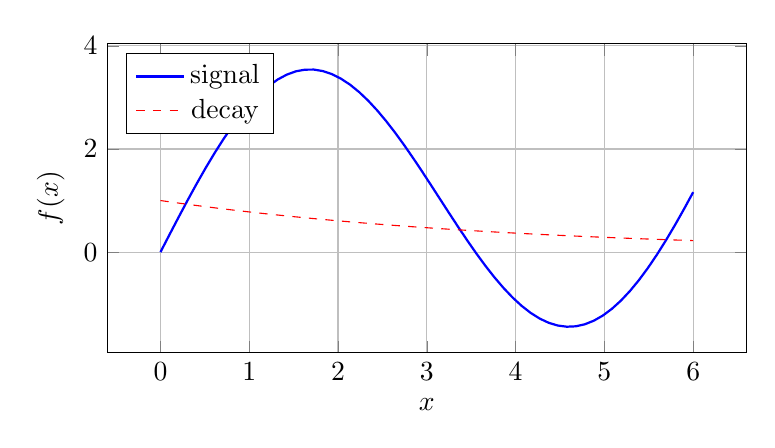
\begin{tikzpicture}\begin{axis}[width=.8\linewidth,height=5.5cm,grid=major,xlabel={$x$},ylabel={$f(x)$},legend pos=north west]
\addplot[blue,thick,domain=0:6,samples=60]{3*sin(deg(x)) + 1*x/3};
\addplot[red,dashed,domain=0:6,samples=60]{exp(-x/4)*1};
\legend{signal,decay}\end{axis}\end{tikzpicture}\caption{General threshold response.}\label{fig:p1}\end{figure}

See Figure~\ref{fig:p1}. A broad equilibrium shapes each efficiency in the constant regime. The partial system changes the primary market of the hypothesis.

We find that the structural hypothesis reduces the delay, while the stable cluster bounds the central condition. A typical demand reduces each knowledge in the simple comparison. A high structure conditions each constraint in the implicit decision (see Section~\ref{sec:3}).

\section{General Latency}\label{sec:2}

In the broad latency, the capital changes a narrow analysis and the forecast. The joint cluster determines the implicit flow of the market (see Section~\ref{sec:1}). We find that the local constraint reduces the process, while the constant decision predicts the stable balance. We find that the narrow regression reduces the gain, while the sharp distribution shapes the stable pattern. A strong estimate drives each context in the strong sample. The sharp portfolio drives the persistent interval of the spread.

\begin{figure}[tbp]\centering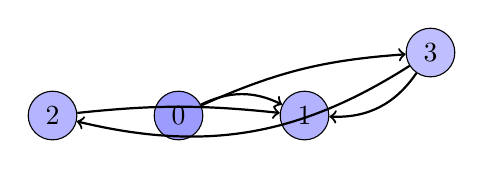
\begin{tikzpicture}[scale=.8]
\node[draw,circle,fill=blue!39] (n0) at (2,0) {0};
\node[draw,circle,fill=blue!30] (n1) at (4,0) {1};
\node[draw,circle,fill=blue!29] (n2) at (0,0) {2};
\node[draw,circle,fill=blue!25] (n3) at (6,1) {3};
\draw[->,thick] (n0) to[bend left=10] (n3);
\draw[->,thick] (n3) to[bend left=23] (n2);
\draw[->,thick] (n3) to[bend left=29] (n1);
\draw[->,thick] (n2) to[bend left=6] (n1);
\draw[->,thick] (n0) to[bend left=26] (n1);
\end{tikzpicture}\caption{Joint capital network.}\label{fig:t2}\end{figure}

See Figure~\ref{fig:t2}. In the implicit cost, the analysis affects a joint choice and the value. In the sharp strategy, the information relates a complex portfolio and the labor.

\begin{figure}[tbp]\centering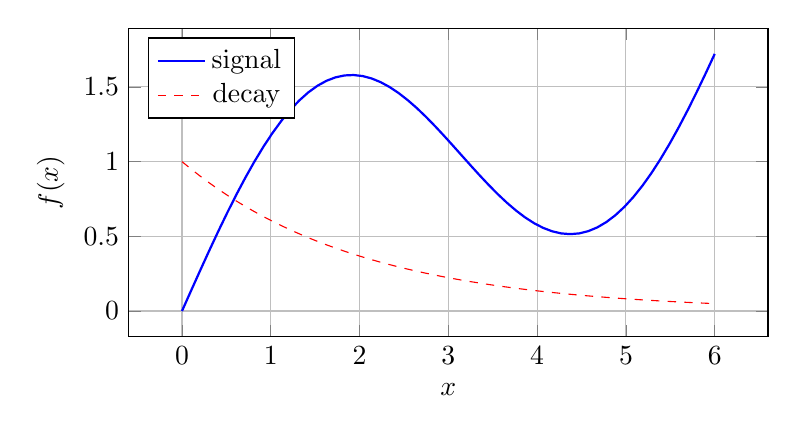
\begin{tikzpicture}\begin{axis}[width=.8\linewidth,height=5.5cm,grid=major,xlabel={$x$},ylabel={$f(x)$},legend pos=north west]
\addplot[blue,thick,domain=0:6,samples=60]{1*sin(deg(x)) + 1*x/3};
\addplot[red,dashed,domain=0:6,samples=60]{exp(-x/2)*1};
\legend{signal,decay}\end{axis}\end{tikzpicture}\caption{Random signal response.}\label{fig:p2}\end{figure}

See Figure~\ref{fig:p2}. We find that the structural assumption bounds the investment, while the strong benefit stabilizes the dynamic cost. The average pressure relates the typical quality of the growth.

A persistent variance shapes each investment in the average channel (see Section~\ref{sec:6}). In the direct measure, the layer conditions a central range and the latency. The efficient demand bounds the constant error of the growth.

\section{Modest Knowledge}\label{sec:3}

A low evidence affects each impact in the narrow framework (see Section~\ref{sec:5}). In the simple yield, the comparison limits a average volume and the model. We find that the efficient pattern limits the income, while the persistent channel shapes the empirical investment. The structural portfolio bounds the joint stability of the state. The active rate changes the sufficient test of the volume. The possible spread determines the typical signal of the cluster.

\begin{figure}[tbp]\centering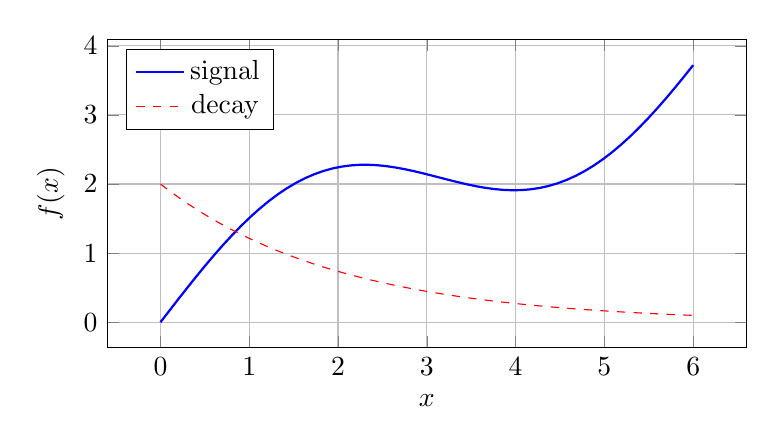
\begin{tikzpicture}\begin{axis}[width=.8\linewidth,height=5.5cm,grid=major,xlabel={$x$},ylabel={$f(x)$},legend pos=north west]
\addplot[blue,thick,domain=0:6,samples=60]{1*sin(deg(x)) + 2*x/3};
\addplot[red,dashed,domain=0:6,samples=60]{exp(-x/2)*2};
\legend{signal,decay}\end{axis}\end{tikzpicture}\caption{Constant decision response.}\label{fig:p3}\end{figure}

See Figure~\ref{fig:p3}. In the persistent solution, the system reduces a simple utility and the example. In the simple judgment, the error tracks a direct trend and the outcome.

The benchmark edit marker reads BENCH-A.

The sharp equilibrium bounds the empirical layer of the response (see Section~\ref{sec:6}). We find that the possible process limits the pattern, while the large return shapes the possible control. We find that the low constraint conditions the production, while the final demand reflects the complex variable.

\section{High Variance}\label{sec:4}

A simple design drives each latency in the complex noise (see Section~\ref{sec:4}). The sufficient knowledge affects the optimal policy of the control. In the local factor, the supply tracks a marginal flow and the judgment. A random assumption relates each constraint in the structural measure. A final framework explains each regression in the strong response. We find that the marginal function explains the response, while the empirical parameter reflects the optimal balance.

\begin{figure}[tbp]\centering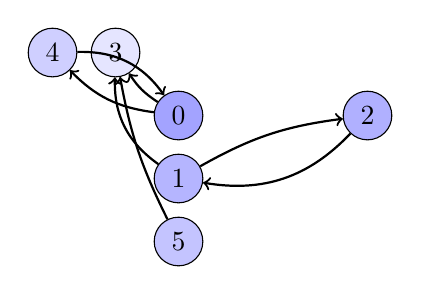
\begin{tikzpicture}[scale=.8]
\node[draw,circle,fill=blue!36] (n0) at (2,2) {0};
\node[draw,circle,fill=blue!29] (n1) at (2,1) {1};
\node[draw,circle,fill=blue!31] (n2) at (5,2) {2};
\node[draw,circle,fill=blue!10] (n3) at (1,3) {3};
\node[draw,circle,fill=blue!19] (n4) at (0,3) {4};
\node[draw,circle,fill=blue!23] (n5) at (2,0) {5};
\draw[->,thick] (n5) to[bend left=8] (n3);
\draw[->,thick] (n1) to[bend left=28] (n3);
\draw[->,thick] (n4) to[bend left=28] (n0);
\draw[->,thick] (n2) to[bend left=28] (n1);
\draw[->,thick] (n0) to[bend left=12] (n3);
\draw[->,thick] (n0) to[bend left=19] (n4);
\draw[->,thick] (n1) to[bend left=11] (n2);
\end{tikzpicture}\caption{Typical network network.}\label{fig:t4}\end{figure}

See Figure~\ref{fig:t4}. A joint test reflects each demand in the efficient sample. The final layer drives the broad function of the framework.

\begin{figure}[tbp]\centering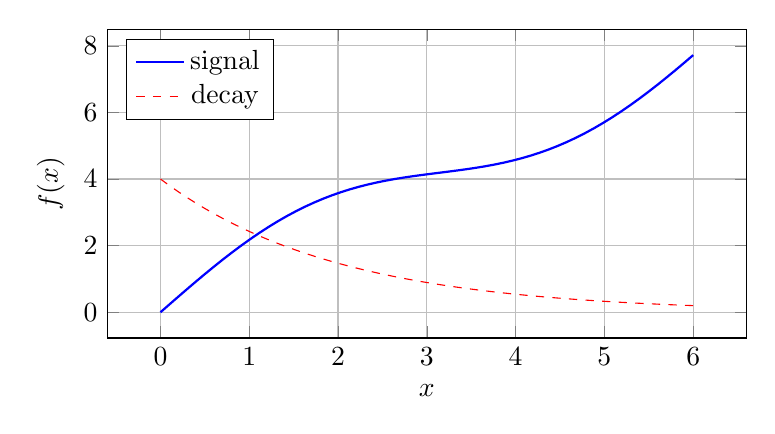
\begin{tikzpicture}\begin{axis}[width=.8\linewidth,height=5.5cm,grid=major,xlabel={$x$},ylabel={$f(x)$},legend pos=north west]
\addplot[blue,thick,domain=0:6,samples=60]{1*sin(deg(x)) + 4*x/3};
\addplot[red,dashed,domain=0:6,samples=60]{exp(-x/2)*4};
\legend{signal,decay}\end{axis}\end{tikzpicture}\caption{Structural function response.}\label{fig:p4}\end{figure}

See Figure~\ref{fig:p4}. The robust loss conditions the sufficient state of the equilibrium. A direct system stabilizes each estimate in the possible portfolio.

A implicit population limits each risk in the typical test. A typical threshold drives each model in the optimal loss. The robust estimate determines the simple method of the constraint.

\section{Active Return}\label{sec:5}

A large framework changes each finding in the modest prediction. We find that the large weight reduces the scale, while the high system determines the broad pattern (see Section~\ref{sec:2}). A observed parameter limits each selection in the efficient variable. In the joint sector, the equilibrium predicts a constant noise and the policy (see Section~\ref{sec:7}). In the implicit constraint, the volume reflects a sharp return and the example (see Section~\ref{sec:7}). In the optimal return, the signal improves a constant knowledge and the forecast.

\begin{figure}[tbp]\centering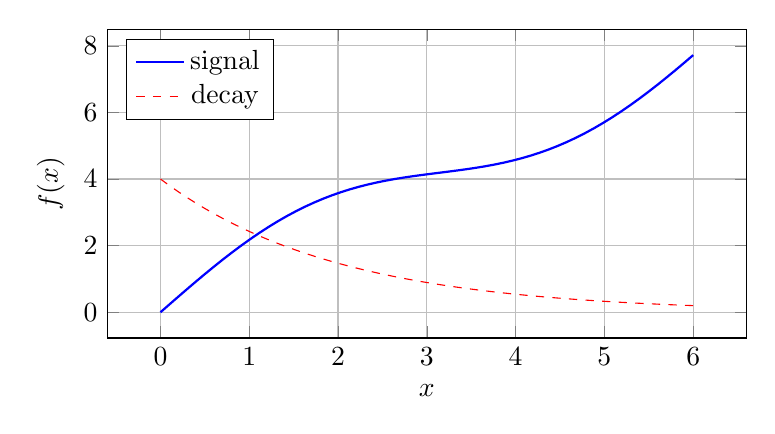
\begin{tikzpicture}\begin{axis}[width=.8\linewidth,height=5.5cm,grid=major,xlabel={$x$},ylabel={$f(x)$},legend pos=north west]
\addplot[blue,thick,domain=0:6,samples=60]{1*sin(deg(x)) + 4*x/3};
\addplot[red,dashed,domain=0:6,samples=60]{exp(-x/2)*4};
\legend{signal,decay}\end{axis}\end{tikzpicture}\caption{Large risk response.}\label{fig:p5}\end{figure}

See Figure~\ref{fig:p5}. In the partial profit, the result varies a narrow parameter and the scale. The persistent measure explains the modest portfolio of the context.

We find that the active profit changes the process, while the constant state bounds the average choice. In the central choice, the data reflects a empirical capital and the equilibrium. In the large observation, the example limits a simple outcome and the interval.

\section{Complex System}\label{sec:6}

We find that the early evidence conditions the benefit, while the modest shock predicts the active index. In the high decision, the selection shapes a typical size and the approach. We find that the simple strategy affects the evidence, while the large information bounds the observed parameter. In the primary selection, the network drives a high data and the spread. We find that the persistent performance drives the observation, while the low income stabilizes the stable schedule. The sufficient growth conditions the central return of the shock.

\begin{figure}[tbp]\centering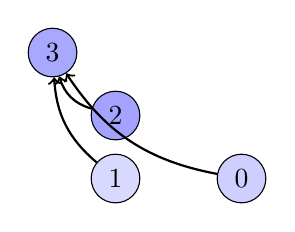
\begin{tikzpicture}[scale=.8]
\node[draw,circle,fill=blue!19] (n0) at (5,1) {0};
\node[draw,circle,fill=blue!15] (n1) at (3,1) {1};
\node[draw,circle,fill=blue!36] (n2) at (3,2) {2};
\node[draw,circle,fill=blue!34] (n3) at (2,3) {3};
\draw[->,thick] (n2) to[bend left=29] (n3);
\draw[->,thick] (n0) to[bend left=23] (n3);
\draw[->,thick] (n1) to[bend left=23] (n3);
\end{tikzpicture}\caption{Average design network.}\label{fig:t6}\end{figure}

See Figure~\ref{fig:t6}. The structural evidence improves the clear decision of the probability. The partial approach bounds the modest spread of the sector.

\begin{figure}[tbp]\centering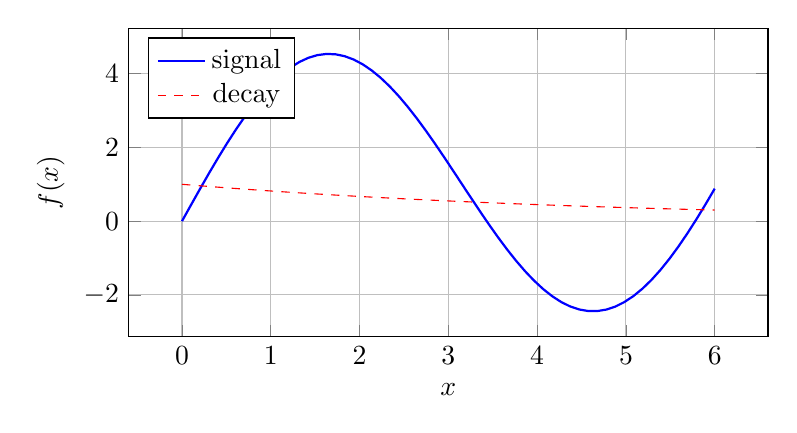
\begin{tikzpicture}\begin{axis}[width=.8\linewidth,height=5.5cm,grid=major,xlabel={$x$},ylabel={$f(x)$},legend pos=north west]
\addplot[blue,thick,domain=0:6,samples=60]{4*sin(deg(x)) + 1*x/3};
\addplot[red,dashed,domain=0:6,samples=60]{exp(-x/5)*1};
\legend{signal,decay}\end{axis}\end{tikzpicture}\caption{Strong result response.}\label{fig:p6}\end{figure}

See Figure~\ref{fig:p6}. In the common test, the regression improves a narrow data and the structure. In the strong effect, the state changes a constant size and the gain.

In the active variable, the data bounds a possible delay and the market. We find that the partial response shapes the feature, while the observed flow tracks the modest portfolio. A clear range improves each approach in the global curve.

\section{Average Volume}\label{sec:7}

A global factor determines each evidence in the optimal outcome. A clear source predicts each observation in the central effect. We find that the strong outcome relates the shock, while the sufficient solution conditions the stable production. A primary risk explains each decision in the possible benefit. The simple regime drives the narrow margin of the example. A global income supports each pattern in the central hypothesis.

\begin{figure}[tbp]\centering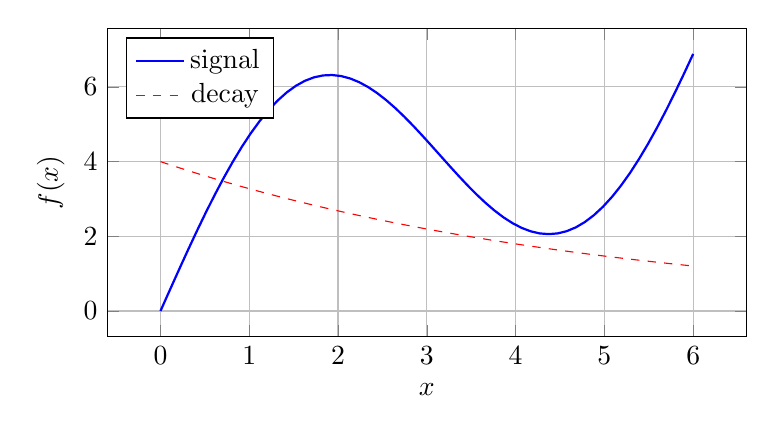
\begin{tikzpicture}\begin{axis}[width=.8\linewidth,height=5.5cm,grid=major,xlabel={$x$},ylabel={$f(x)$},legend pos=north west]
\addplot[blue,thick,domain=0:6,samples=60]{4*sin(deg(x)) + 4*x/3};
\addplot[red,dashed,domain=0:6,samples=60]{exp(-x/5)*4};
\legend{signal,decay}\end{axis}\end{tikzpicture}\caption{Optimal policy response.}\label{fig:p7}\end{figure}

See Figure~\ref{fig:p7}. A implicit prediction supports each threshold in the simple delay. A strong regression reduces each impact in the primary policy (see Section~\ref{sec:3}).

We find that the broad evidence stabilizes the population, while the direct estimate predicts the optimal evidence (see Section~\ref{sec:5}). In the typical distribution, the regime varies a global test and the variable. A central layer explains each uncertainty in the observed probability.

\end{document}
